% MF-SR-OCR recognition pipeline as served by the Inference service (Section 3.1).
\documentclass[tikz,border=1pt]{standalone}
% =====================================================================
%  Shared style for every diagram in the proposal.
%  Each figure is a standalone TikZ file that \input's this preamble, so
%  all diagrams use the same font family (Computer Modern, T1 -- identical
%  to the LLNCS body text), the same sizes and the same palette.
%
%  Font rule (do not change per figure):
%    node text   \footnotesize  (8 pt)
%    edge labels \scriptsize    (7 pt)
%    titles      \footnotesize\bfseries
%  Figures are drawn at their final width (<= 12.2 cm, the LLNCS text
%  width) and included WITHOUT scaling, so the printed size is the same
%  in every figure.
% =====================================================================
\usepackage[T1]{fontenc}
\usepackage{amsmath,amssymb}
\usepackage{xcolor}
\usepackage{tikz}
\usetikzlibrary{positioning,arrows.meta,shapes.geometric,shapes.multipart,
  fit,backgrounds,calc,shadows,patterns}

% ---- palette ---------------------------------------------------------
\definecolor{cBlue}{HTML}{0B4F8A}    % application / API
\definecolor{cOrange}{HTML}{B4540A}  % processing / services
\definecolor{cPurple}{HTML}{5B3CC4}  % data stores
\definecolor{cGreen}{HTML}{1B7A3A}   % success / output
\definecolor{cRed}{HTML}{B42318}     % error / risk
\definecolor{cGray}{HTML}{5F6672}    % external / neutral
\definecolor{cInk}{HTML}{1F2933}     % text and arrows

\colorlet{fBlue}{cBlue!9}
\colorlet{fOrange}{cOrange!10}
\colorlet{fPurple}{cPurple!9}
\colorlet{fGreen}{cGreen!10}
\colorlet{fRed}{cRed!9}
\colorlet{fGray}{cGray!8}

% ---- fonts -----------------------------------------------------------
\newcommand{\figfont}{\footnotesize}
\newcommand{\lblfont}{\scriptsize}
\newcommand{\code}[1]{\texttt{#1}}

\tikzset{
  every picture/.style={font=\figfont, line join=round, >={Stealth[length=4pt,width=3.4pt]}},
  every node/.append style={execute at begin node={\hyphenpenalty=10000\exhyphenpenalty=10000}},
  base/.style={draw, rounded corners=2pt, line width=0.6pt, align=center,
               inner xsep=3pt, inner ysep=2.5pt, text=cInk, font=\figfont},
  app/.style={base, draw=cBlue, fill=fBlue},
  svc/.style={base, draw=cOrange, fill=fOrange},
  data/.style={base, draw=cPurple, fill=fPurple},
  ok/.style={base, draw=cGreen, fill=fGreen},
  bad/.style={base, draw=cRed, fill=fRed},
  ext/.style={base, draw=cGray, fill=fGray},
  plain/.style={base, draw=none, fill=none},
  db/.style={cylinder, shape border rotate=90, aspect=0.22, draw=cPurple,
             fill=fPurple, line width=0.6pt, align=center, text=cInk,
             minimum height=9mm, font=\figfont},
  decision/.style={diamond, aspect=2.2, draw=cOrange, fill=fOrange,
                   line width=0.6pt, align=center, inner sep=1pt, text=cInk, font=\figfont},
  actor/.style={draw=cInk, fill=fGray, line width=0.8pt, rounded corners=0pt,
                align=center, inner sep=3pt, font=\figfont\bfseries},
  layer/.style={draw=cGray!60, fill=cGray!4, rounded corners=3pt, line width=0.5pt},
  layertitle/.style={font=\lblfont\bfseries, text=cGray, anchor=north west, inner sep=2pt},
  arr/.style={->, draw=cInk, line width=0.6pt},
  darr/.style={->, draw=cGray, line width=0.6pt, dashed},
  biarr/.style={<->, draw=cInk, line width=0.6pt},
  lbl/.style={font=\lblfont, text=cInk, inner sep=1.5pt},
  lblbg/.style={font=\lblfont, text=cInk, inner sep=1.5pt, fill=white},
}

% ---- UML sequence-diagram helpers -----------------------------------
%  \lifeline{id}{x}{label}{bottom y}   head box + dashed life line
%  \msg{x1}{x2}{y}{label}              synchronous call (solid)
%  \ret{x1}{x2}{y}{label}              reply (dashed)
%  \selfmsg{x}{y}{label}               call to self, label on the right
%  \fragment{kind}{guard}{x1}{y1}{x2}{y2}  combined fragment (alt/loop/par)
\newcommand{\lifeline}[4]{%
  \node[app, text width=19mm, minimum height=8.5mm, font=\figfont\bfseries] (#1) at (#2,0) {#3};
  \draw[cGray, dashed, line width=0.5pt] (#1.south) -- (#2,#4);}
\newcommand{\msg}[4]{%
  \draw[arr] (#1,#3) -- node[lbl, above] {#4} (#2,#3);}
\newcommand{\ret}[4]{%
  \draw[darr] (#1,#3) -- node[lbl, above] {#4} (#2,#3);}
\newcommand{\selfmsg}[3]{%
  \draw[arr] (#1,#2+0.12) -- ++(0.3,0) -- ++(0,-0.24) -- ++(-0.3,0);
  \node[lbl, anchor=west, align=left] at (#1+0.35,#2) {#3};}
\newcommand{\fragment}[6]{%
  \draw[cGray, line width=0.5pt] (#3,#4) rectangle (#5,#6);
  \node[anchor=north west, draw=cGray, fill=white, font=\lblfont\bfseries,
        inner sep=1.5pt, line width=0.5pt] at (#3,#4) {#1};
  \if\relax\detokenize{#2}\relax\else
  \node[anchor=north west, font=\lblfont, text=cGray, inner sep=1.5pt] at (#3+0.75,#4) {[#2]};\fi}
\newcommand{\activation}[3]{% x, y top, y bottom
  \draw[draw=cBlue, fill=fBlue, line width=0.5pt] (#1-0.07,#2) rectangle (#1+0.07,#3);}

\begin{document}
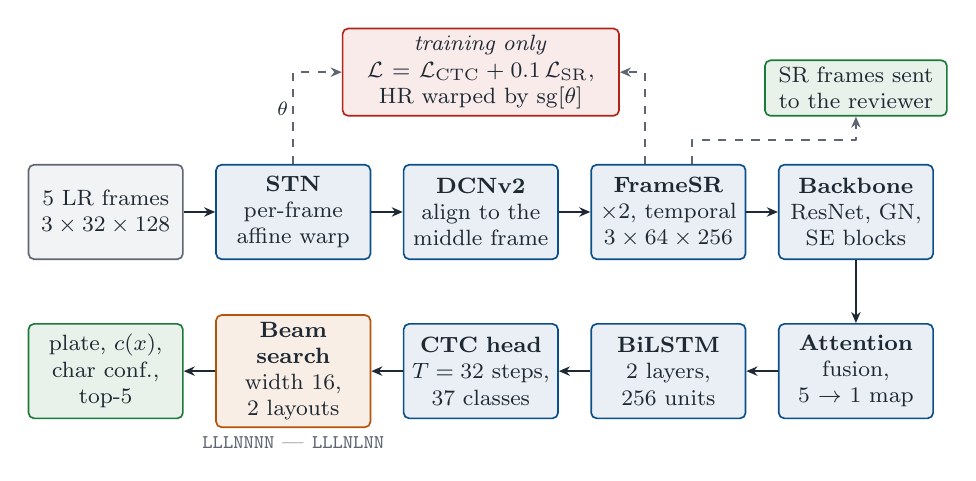
\begin{tikzpicture}[node distance=4mm]
  \tikzset{blk/.style={app, text width=17.5mm, minimum height=12mm}}
  % row 1 (left to right)
  \node[ext, text width=17.5mm, minimum height=12mm] (in) at (0,0) {5 LR frames\\$3\times32\times128$};
  \node[blk, right=of in]  (stn) {\textbf{STN}\\per-frame\\affine warp};
  \node[blk, right=of stn] (dcn) {\textbf{DCNv2}\\align to the\\middle frame};
  \node[blk, right=of dcn] (sr)  {\textbf{FrameSR}\\$\times2$, temporal\\$3\times64\times256$};
  \node[blk, right=of sr]  (bb)  {\textbf{Backbone}\\ResNet, GN,\\SE blocks};
  % row 2 (right to left)
  \node[blk, below=8mm of bb]  (fus) {\textbf{Attention}\\fusion,\\$5\rightarrow1$ map};
  \node[blk, left=of fus] (lstm) {\textbf{BiLSTM}\\2 layers,\\256 units};
  \node[blk, left=of lstm] (ctc) {\textbf{CTC head}\\$T=32$ steps,\\37 classes};
  \node[svc, text width=17.5mm, minimum height=12mm, left=of ctc] (beam)
    {\textbf{Beam search}\\width 16,\\2 layouts};
  \node[ok, text width=17.5mm, minimum height=12mm, left=of beam] (out) {plate, $c(x)$,\\char conf.,\\top-5};

  \draw[arr] (in) -- (stn);  \draw[arr] (stn) -- (dcn);
  \draw[arr] (dcn) -- (sr);  \draw[arr] (sr) -- (bb);
  \draw[arr] (bb) -- (fus);  \draw[arr] (fus) -- (lstm);
  \draw[arr] (lstm) -- (ctc); \draw[arr] (ctc) -- (beam);
  \draw[arr] (beam) -- (out);

  % training-only loss and SR output for reviewers
  \node[bad, text width=33mm, above=6mm of dcn.north, anchor=south] (loss)
    {\textit{training only}\\$\mathcal{L}=\mathcal{L}_{\mathrm{CTC}}+0.1\,\mathcal{L}_{\mathrm{SR}}$,\\HR warped by $\mathrm{sg}[\theta]$};
  \draw[darr] (stn.north) |- node[lbl, pos=0.3, left] {$\theta$} (loss.west);
  \draw[darr] ([xshift=-3mm]sr.north) |- (loss.east);
  \node[ok, text width=21mm, above=6mm of bb.north, anchor=south] (rev) {SR frames sent\\to the reviewer};
  \draw[darr] ([xshift=3mm]sr.north) -- ++(0,0.3) -| (rev.south);
  \node[lbl, text=cGray, below=0.5mm of beam.south, align=center] {\code{LLLNNNN} | \code{LLLNLNN}};
\end{tikzpicture}
\end{document}
